\documentclass{standalone}
\usepackage{tikz}
\usetikzlibrary{patterns}
\usepackage{pgfplots}
\usepackage{pgfplotstable}
\begin{document}%
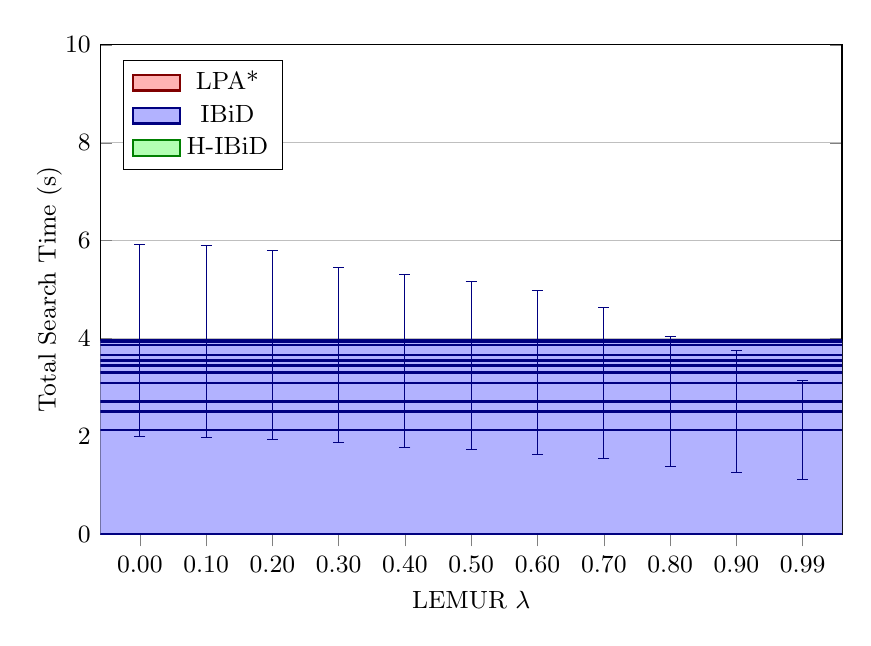
\begin{tikzpicture}[font=\small]

\ifdefined\arghideibid
\else
   \def\drawhideibid{}
\fi

% for herbbookshelfnom problem, lemur (not family)

% $ rosrun thesis_experiments txt-sql.py
%   --select=param --select=planner-dur-search-finmean --select=planner-dur-search-stderrfinmean
%   < multistep-prescribed/results/stats-byparam-herbbookshelfnom-lemur-lpastar-haltonoffdens10000,1.0-lambda.txt
\pgfplotstableread{
lambda mean meanstderr
0.00 0.9840960197599997 0.26979778672996707
0.10 0.9593325140400001 0.25243647291051224
0.20 1.0120981483200004 0.26784954256203003
0.30 1.0489787729200004 0.26691246811141517
0.40 1.1508470771799997 0.29421027152098356
0.50 1.2831634680000001 0.33869347591018273
0.60 1.4953775792799993 0.40282301842936813
0.70 1.9981444564400008 0.5924133811175923
0.80 2.8321833429199996 0.9645373690326533
0.90 4.844260971840002 1.942441768713175
0.99 8.506768436999998 3.761253254868455
}{\datalpastar}

% 1.96* stderr fill loop
\pgfplotstableread{
lambda meanpm
0.00 1.5128996817507352
0.10 1.4541080009446041
0.20 1.5370832517415793
0.30 1.572127210418374
0.40 1.7274992093611274
0.50 1.9470026807839584
0.60 2.2849106954015608
0.70 3.159274683430482
0.80 4.722676586224
0.90 8.651446838517824
0.99 15.87882481654217
0.99 1.1347120574578264
0.90 1.0370751051621787
0.80 0.9416900996159991
0.70 0.8370142294495198
0.60 0.7058444631584377
0.50 0.619324255216042
0.40 0.5741949449988719
0.30 0.5258303354216267
0.20 0.48711304489842155
0.10 0.4645570271353961
0.00 0.45529235776926424
}{\datalpastarloop}

% $ rosrun thesis_experiments txt-sql.py
%   --select=param --select=planner-dur-search-finmean --select=planner-dur-search-stderrfinmean
%   < multistep-prescribed/results/stats-byparam-herbbookshelfnom-lemur-incbi-haltonoffdens10000,1.0-lambda.txt
\pgfplotstableread{
lambda mean meanstderr
0.00 3.9616373558799993 0.998229149264443
0.10 3.9397860089200005 0.9990470383089352
0.20 3.871332568659999 0.9818551714837519
0.30 3.663623169000001 0.9133215204893451
0.40 3.5527050717800006 0.9009538133731313
0.50 3.4527792869000002 0.8740585266460358
0.60 3.309325582719999 0.8522247215298356
0.70 3.0923112411399996 0.7874416494948657
0.80 2.7163222726799994 0.6749227256964755
0.90 2.5112581661199997 0.6391571756073432
0.99 2.13875917712 0.5181582097408343
}{\dataibid}

% 1.96* stderr fill loop
\pgfplotstableread{
lambda meanpm
0.00	5.918166488438308
0.10	5.897918204005514
0.20	5.795768704768152
0.30	5.453733349159117
0.40	5.318574545991337
0.50	5.1659339991262305
0.60	4.979686036918477
0.70	4.635696874149936
0.80	4.039170815045091
0.90	3.7640062303103923
0.99	3.154349268212035
0.99	1.1231690860279646
0.90	1.258510101929607
0.80	1.3934737303149074
0.70	1.5489256081300629
0.60	1.6389651285215214
0.50	1.7396245746737702
0.40	1.7868355975686634
0.30	1.8735129888408846
0.20	1.9468964325518452
0.10	1.9816538138344877
0.00	2.0051082233216913
}{\dataibidloop}

% $ rosrun thesis_experiments txt-sql.py
%   --select=param --select=planner-dur-search-finmean --select=planner-dur-search-stderrfinmean
%   < multistep-prescribed/results/stats-byparam-herbbookshelfnom-lemur-wincbi-haltonoffdens10000,1.0-lambda.txt
\pgfplotstableread{
lambda mean meanstderr
0.00 2.7052947179999993 0.6436018181240384
0.10 2.59071953508 0.626001750866798
0.20 2.49428646288 0.5913381574283408
0.30 2.5211604733999993 0.6027475795307445
0.40 2.43547666178 0.5840600392544062
0.50 2.42686321534 0.5930127292495511
0.60 2.41011039842 0.5924946671135987
0.70 2.3683262786999997 0.5833656264353004
0.80 2.3788538110399995 0.5674139870644058
0.90 2.65935832118 0.7078099309313812
0.99 3.0323717004400006 0.8180209188182312
}{\datahibid}

% 1.96* stderr fill loop
\pgfplotstableread{
lambda meanpm
0.00	3.9667542815231145
0.10	3.817682966778924
0.20	3.653309251439548
0.30	3.7025457292802586
0.40	3.580234338718636
0.50	3.58916816466912
0.60	3.5713999459626535
0.70	3.5117229065131887
0.80	3.490985225686235
0.90	4.046665785805507
0.99	4.635692701323734
0.99	1.4290506995562673
0.90	1.2720508565544928
0.80	1.2667223963937642
0.70	1.2249296508868108
0.60	1.2488208508773466
0.50	1.26455826601088
0.40	1.290718984841364
0.30	1.33977521751974
0.20	1.3352636743204518
0.10	1.363756103381076
0.00	1.4438351544768842
}{\datahibidloop}

\begin{axis}[
   width=11cm,
   height=7.8cm,
   ybar=0pt,
   bar width=6,
   ymin=0,ymax=10,
   %xmin=-0.05, xmax=1.05,
   enlarge x limits={abs=0.5cm},
   %xmin=0,xmax=95,
   %xtick pos=bottom,
   %symbolic y coords={E, F, R, A, B, W, P},
   xticklabels from table={\datalpastar}{lambda},
   xtick=data,
   xtick pos=left,
   ymajorgrids,
   %xmajorticks=false,
   %ticklabel style={font=\footnotesize},
   %xticklabel style={rotate=20},
   %xticklabel shift=-0.1cm,
   ylabel={Total Search Time (s)},
   ylabel near ticks,
   ylabel shift=-0.2cm,
   xlabel={LEMUR $\lambda$},
   legend pos=north west,
   x dir=reverse,
   %reverse legend,
   %legend style={font=\footnotesize},
   ]

\addplot[color=red!50!black,fill=red!30,area legend,thick,error bars/.cd,y dir=both,y explicit]
   table[x expr=1-0.1*\coordindex,y=mean,y error expr=1.96*\thisrow{meanstderr}]
   {\datalpastar};
\addlegendentry{LPA*};

\ifdefined\drawhideibid

\addplot[color=blue!50!black,fill=blue!30,area legend,thick,error bars/.cd,y dir=both,y explicit]
   table[x expr=1-0.1*\coordindex,y=mean,y error expr=1.96*\thisrow{meanstderr}]
   {\dataibid};
\addlegendentry{IBiD};

\addplot[color=green!50!black,fill=green!30,area legend,thick,error bars/.cd,y dir=both,y explicit]
   table[x expr=1-0.1*\coordindex,y=mean,y error expr=1.96*\thisrow{meanstderr}]
   {\datahibid};
\addlegendentry{H-IBiD};

\fi

%\begin{axis}[
%   width=11cm,
%   height=7.8cm,
%   %ybar=0pt,
%   %bar width=6,
%   ymin=0,
%   %xmin=-0.05, xmax=1.05,
%   enlarge x limits={abs=0.5cm},
%   %xmin=0,xmax=95,
%   %xtick pos=bottom,
%   %symbolic y coords={E, F, R, A, B, W, P},
%   %xticklabels from table={\datainit}{barname},
%   %xtick=data,
%   %xtick pos=left,
%   ymajorgrids,
%   %xmajorticks=false,
%   %ticklabel style={font=\footnotesize},
%   %xticklabel style={rotate=20},
%   %xticklabel shift=-0.1cm,
%   ylabel={Total Search Time (s)},
%   ylabel near ticks,
%   %ylabel shift=-0.2cm,
%   legend pos=north west,
%   %reverse legend,
%   %legend style={font=\footnotesize},
%   ]
%
%\addplot
%   plot[mark=none,color=red!20,fill=red!40,fill opacity=0.8]
%   table[x=lambda,y=meanpm]
%   {\datalpastarloop};
%
%\addplot
%   plot[mark=none,color=blue!20,fill=blue!40,fill opacity=0.5]
%   table[x=lambda,y=meanpm]
%   {\dataibidloop};
%
%\addplot
%   plot[mark=none,color=green!20,fill=green!10,fill opacity=0.5]
%   table[x=lambda,y=meanpm]
%   {\datahibidloop};
%
%\addplot[color=red,area legend,thick,error bars/.cd,y dir=both,y explicit]
%   table[x=lambda,y=mean,y error expr=1.96*\thisrow{meanstderr}]
%   {\datalpastar};
%\addlegendentry{LPA*};
%
%\addplot[color=blue,area legend,thick,error bars/.cd,y dir=both,y explicit]
%   table[x=lambda,y=mean,y error expr=1.96*\thisrow{meanstderr}]
%   {\dataibid};
%\addlegendentry{IBiD};
%
%\addplot[color=green!50!black,area legend,thick,error bars/.cd,y dir=both,y explicit]
%   table[x=lambda,y=mean,y error expr=1.96*\thisrow{meanstderr}]
%   {\datahibid};
%\addlegendentry{H-IBiD};

\end{axis}

\end{tikzpicture}
\end{document}
